\chapter{Data Path Resilience} 

In White Rabbit Network, Data Path Resilience is a prerequisite to the network's
Determinism and Clock Path Resilience. Therefore, it's of utmost importance. 

The requirement regarding Data Path Resilience is simple: loose no more than
single \ControlMessage\ per year. It means that out of all the \ControlMessage
s which are sent every \GranularityWindow\ to \~2000 WR Nodes, only one can be
lost. 
% It translates into reliability of "11 nines" for GSI and "10 nines" for
%CERN (see Table~\ref{tab:requirements}). 


Resilience in White Rabbit is achieved by redundancy. Redundant cabling (fibre
and copper) and network devices (WR Switches, WR Nodes) guarantee physical path
continuity despite network components failure. This redundancy is managed by
Rapid Spanning Tree Protocol (RSPT) to ensure tree-like data path.
Imperfection of physical medium can cause data corruption. Corrupted data
delivered successfully to the destination is rendered useless. This problem can
be overcome by introducing data redundancy through special coding. In White
Rabbit Network, Error Correction is used. However, even highly
redundant network, is considered unreliable if the information is lost (packages
dropped) due to traffic congestion. Therefore, Flow and Congestion Control
require special attention in Data Path Resilience consideration. 

The overall reliability of White Rabbit Network is a combination of the above
mentioned factors. Assuming that 

\begin{itemize}
        \item $P_{congestion}$ is the probability that there is a congestion in
	      the network, and the packages are dropped and \ControlMessage\ is lost,
        \item $P_{f\_FEC}$ is the probability that FEC failed and a
	      \ControlMessage\ delivered to a WR Node cannot be decoded.
        \item $P_{f\_Network}$ is the probability that there is a network
	      failure which prevents a \ControlMessage\ to be delivered to any
	      WR Node
\end{itemize}
 
the probability of WR Network failure is:
\begin{equation}
  \label{equation:WRreliability}
     P_{WRN_f} =  P_{congestion} + P_{f\_FEC} + P_{f\_Network}
\end{equation}
since all the probabilities are independent, the White Rabbit Network
reliability can be calculated:
\begin{equation}
   \label{equation:WRreliability}
      R_{WRN} = 1 - (P_{congestion} + P_{f\_FEC} + P_{f\_Network})
\end{equation}

Since the expected WR Network failure rate is known
(see Table~\ref{tab:requirements}), there are very clear goals to achieve in
terms of Data Path Resilience. 

% ==============================================================================
\section{Rapid Spanning Tree Protocol} 
% ==============================================================================

White Rabbit Networks requires a robust communications network that can avoid 
single points of failures. Redundancy can be used to eliminate network downtime
caused by:
\begin{itemize}
        \item switch breakdown,
        \item port malfunction,
        \item cabling failure.
\end{itemize}
Network components' redundancy provides redundant data links and improve fault
tolerance but it also creates link loop. A broadcast communication in a network
with loops results in a "broadcast storm" where frames circulate around the loop
forever, rendering the network useless.

In order to eliminate loops in the network the Rapid Spanning Tree
Protocol (RSTP) will be used. It is a protocol that allows switches to
communicate with each other to discover physical loops in the network. It then
creates a loop-free logical topology by blocking appropriate switches' ports.

RSTP is included in standard for LAN bridges (IEEE 802.1D \cite{IEEE8021D}). It
is an evolution of the Spanning Tree Protocol (STP) which provides faster
spanning tree convergence after a topology change. For an exhaustive description
of RSTP, read the Appendix~\ref{appD}.


% ==============================================================================
\subsection{White Rabbit Rapid Spanning Tree} 
\label{chapter:WRRSTP}
% ==============================================================================

White Rabbit introduces no changes to Rapid Spanning Tree Protocol and
algorithm. However, it takes advantage of hardware support (e.g.: \HP\ Bypass)
to enhance RSTP convergence performance. The time of original RSTP convergence
differs depending on the network topology, it is important for the reader to
comprehend RSTP convergence mechanism in order to understand the proposed
solution and limitations of topology. Therefore, RSTP and its convergence are
described in details in Appendix~\ref{appD}. 

The aim of WR Rapid Spanning Tree is three-fold:

\begin{itemize}
  \item Loose no \ControlMessage s during topology change caused by switch or
link failure. It translates into changing topology for \HP\ Traffic within
the length of \HP\ Package transmission time (microseconds).
  \item Prevent the creation of new physical loops when the topologies change.
  \item Enhance the speed of topology change for \SP\ Traffic.
\end{itemize}

Due to its importance, tight latency constraints and separate routing
implementation, \HP\ Traffic needs to be considered separately from \SP\ traffic
for WR RSTP implementation. 

 
% ==============================================================================
\subsubsection{\HighPriority\ Traffic in RSTP } 
% ==============================================================================

In order to meet the requirement of loosing single \ControlMessage\  per year,
the number of lost \HP\ Packages cannot exceed the possibilities of FEC recovery
This depends on FEC's configuration (see Chapter~\ref{chapter:FEC}), we assume
that only single \HP\ package in a burst (the most demanding use case). This 
restriction holds during the process of topology change due to link/switch
failure. If such failure happens during \ControlMessage\  transmission (\HP\
Package burst), the switching to alternative link needs to be quick enough to loose
at most only single \HP\ Package. Since the minimal considered \HP\ Package size
is 500 bytes, the maximum switch-over time is precisely known: it is 3 $\mu s$,
see Table~\ref{tab:FECedSize}. The switch-over time, below-3 $\mu $, exceeds
the possibilities of standard RSTP implementations by orders of magnitudes.
While the standard RSTP implementations provide switch-over time of few seconds,
the shortest switch-over time found in commercial switches is in order of
milliseconds \cite{ciscoRSTP}. This concerns the switch-over in simple cases
(dual-link arrangement).

It needs to be noticed, that the requirement of loosing single \ControlMessage\
per year concerns only \HP\ Traffic, therefore the below-3 $\mu s$ RSTP
switch-over is needed only for \HP\ Packages. This enables to take advantage of
the following features of \HP\ Traffic:
\begin{itemize}
  \item \HP\ Traffic is broadcast, which means that  MAC-address re-learning
	is not required after switch-over.
  \item \HP\ Traffic is routed using \HP\ Bypass, 
	Chapter~\ref{chapter:HPbypass}.
\end{itemize}

Consequently, RSTP switch-over mechanisms for \HP\ Traffic can be
implemented in hardware as an extension to \HP\ Bypass. However, the hardware
implementation can be effectively fast only if alternative ports (links) are
known in advance. By alternative ports we mean ports which are assigned
alternate or backup roles, as defined in IEEE 802.1D standard\cite{IEEE8021D}.
Such ports are identified when the RSTP Algorithm establishes more then one path
to Root Switch of the RSTP Tree topology and both paths can be used
simultaneously (simplified explanation). In example, the proposed method will
work fine with dual-link arrangement, but will fail with ring topology.
Therefore, the suggested solution implies restriction on network topology(see
Figure~\ref{fig:wrRSTPtopologies}):
\begin{itemize}
  \item RSTP Root Switch connected directly to Data Master Node
(this should be enforced by appropriate configuration).
  \item No ring topology arrangement. 
  \item The only possible paths from a non-Root Switch to the Root Switch shall
be through root, alternate or disabled ports. 
  \item A possible path from non-Root Switch to the Root Switch through
designated or backup port (e.g.: ring topology) prevents the proposed solution
to work properly.
  \item Backup RSTP Root Switch(s) is a WR switch connected:
  \begin{itemize}
    \item to Data Master(s) and/or
    \item with two links to RSTP Root Switch and, optionally to Data
	  Master(s).
  \end{itemize} 
\end{itemize}
The above restrictions greatly overlap with restrictions imposed by the
Timing Path Redundancy.

\begin{center}
	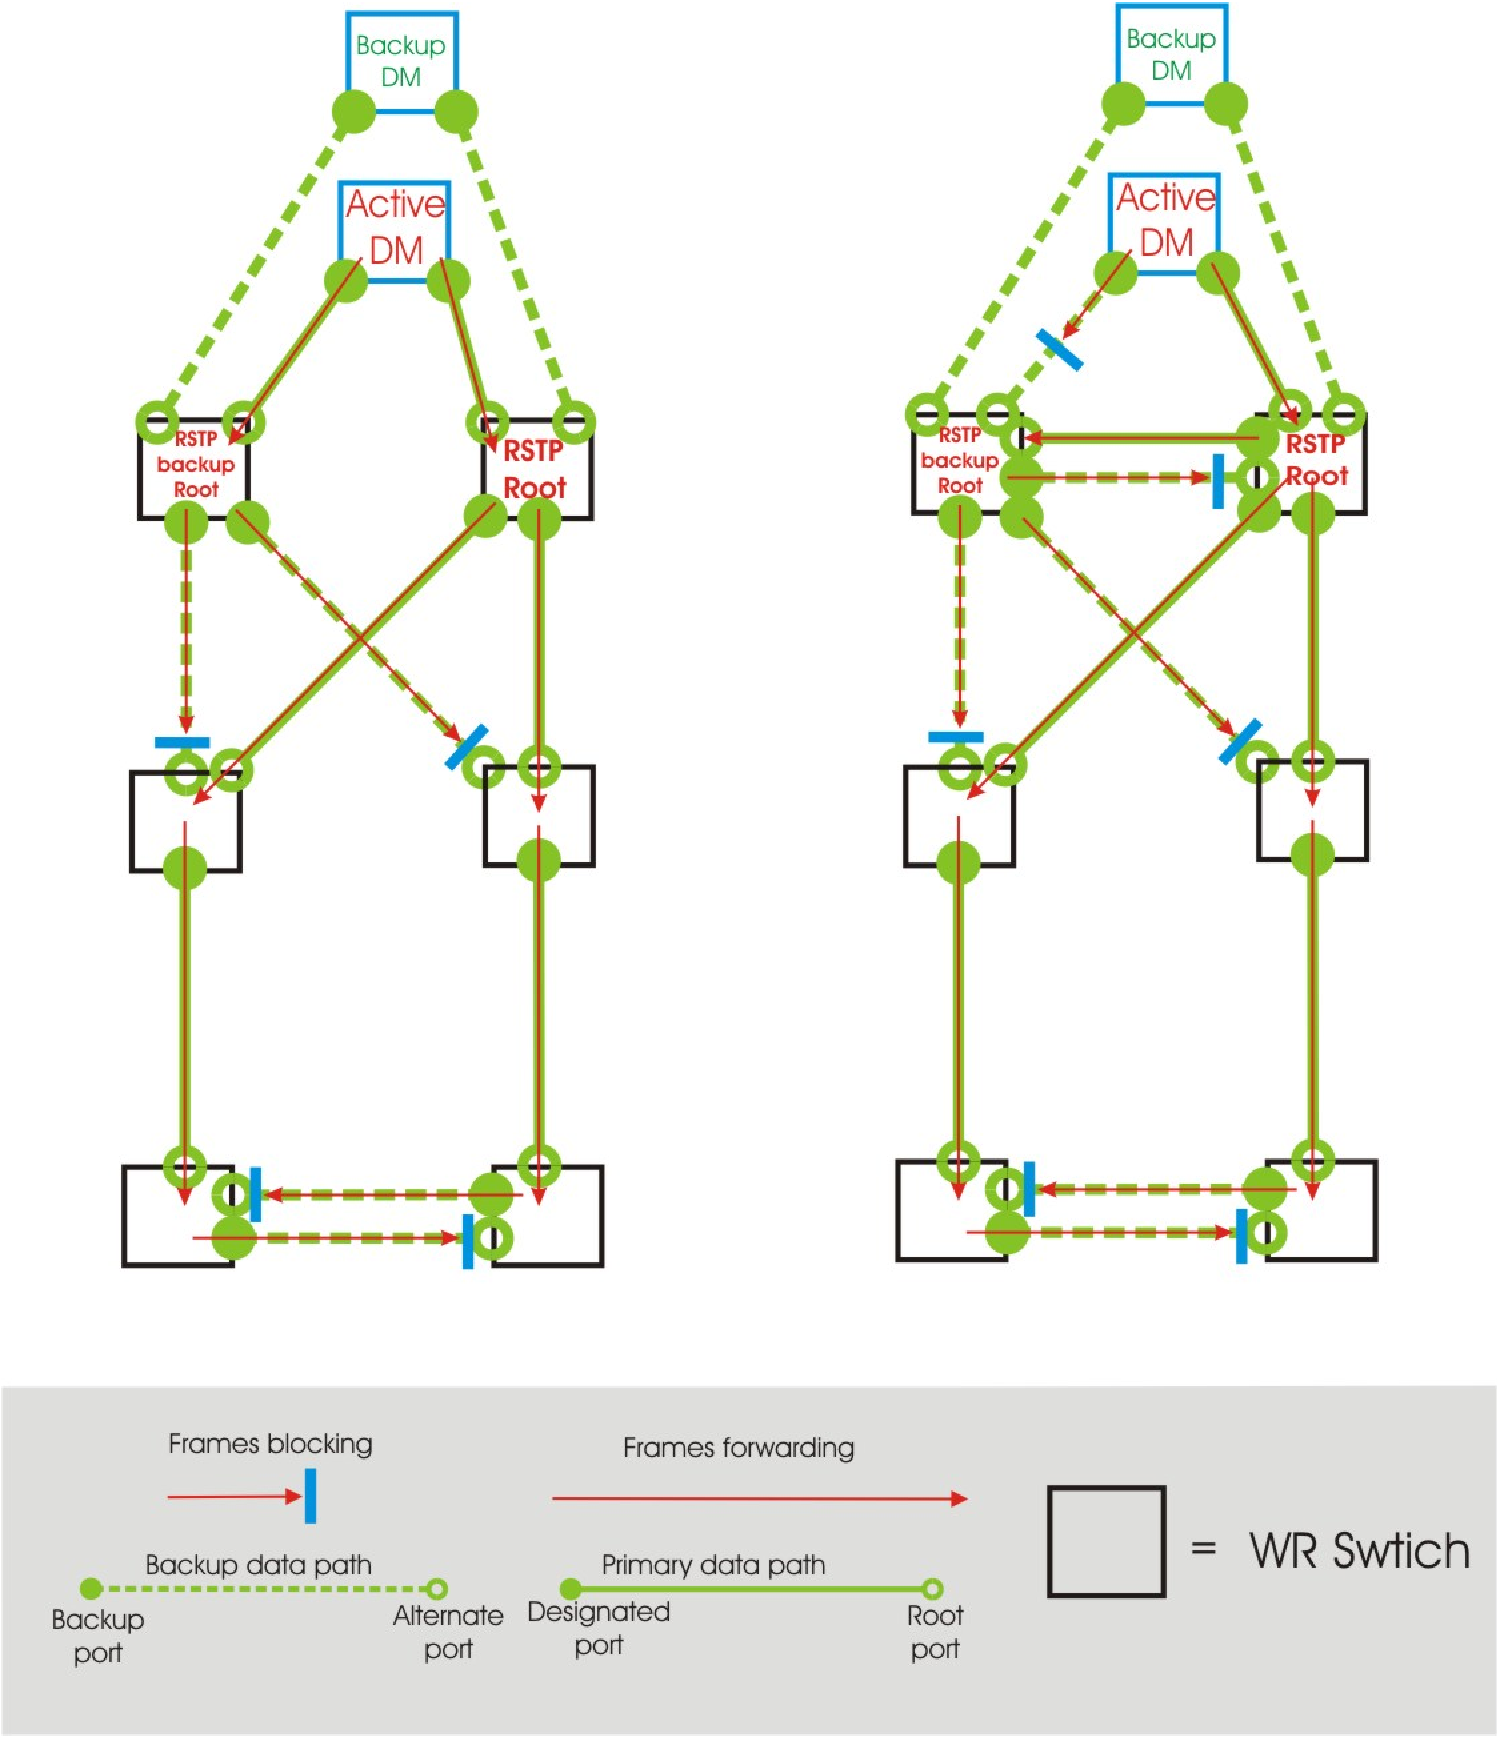
\includegraphics[scale=0.30]{../../../../figures/robustness/wrRSTPtopologies.ps}
	\captionof{figure}{Example of topologies including WR restrictions to
RSTP, highlighting connections between Backup Root Switch, Root Switch and Data
Master(s) Nodes.}
	\label{fig:wrRSTPtopologies}
\end{center}

It is estimated that the switch-over provided by the hardware implementation
for \HP\ Traffic will take an order of few hundred nanoseconds (few cycles). The
estimated time to detect (in hardware) link failure is up to $1\mu s$.
Therefore, it can be assumed that the entire switch-over process shall take
$~1\mu s$, which is sufficient. 

The suggested hardware implementation of the method is included in
Appendix~\ref{appC}. The implementation is meant to relay on the information
provided by RSTP Algorithm and impose no changes to the Algorithm. 
 
Appendix~\ref{appD} includes Use Cases which presents behaviour of the network,
with the proposed solutions, in case of failures of various elements of the
network.

The proposed solution has its limitation, possible solutions to overcome this
shortcomings, to be considered in next version of this doc, are listed in
Appendix~\ref{appD}.

 
% ==============================================================================
\subsubsection {\StandardPriority\ Traffic in RSTP}  
% ==============================================================================

This document (version 1) suggests no special changes to RSTP targeted at
\StandardPriority\ Traffic. The only enhancement is the fact that link failure
is detected in hardware. It should significantly speed up the convergence time.
Additionally, the limitations imposed on the White Rabbit Network Topology,
should ensure reasonably fast RSTP convergence. 

Proposals of WR extension of RSTP to significantly increase RSTP performance
for \StandardPriority Traffic are included in Appendix~\ref{appD}.


% ==============================================================================
\section{Forward Error Correction}
% ==============================================================================
\label{chapter:FEC}

The objective of the Forward Error Correction, FEC, in the White Rabbit Network
is to achieve the loss of one \ControlMessage per year over Ethernet. A
\ControlMessage is wrapped in Ethernet frames, as payload, and sent over a
flawed physical medium. The medium could alter either the payload,
\ControlMessage, or the header of the Ethernet frame resulting in flawed or lost
frame, respectively. By using a FEC scheme the receiver can repair an error
in the original frame as long as redundant information was added, and the loss
of a frame if the information plus redundant information was sent in several
frames. The next chapters analyze the WR Network regarding the BER, the
topology and destination address of the frame. The outcome will indicate which
kind of FEC we shall use and the redundancy needed. Finally a use case will be
presented in order to illustrate how this mechanism will guarantee the
requirement.

\subsection{Physical Medium, BER and Communication Channel in WR Network} 

White Rabbit uses as a physical medium, Fiber Optic and CAT-5. These
mediums are flawed and noisy, and can introduce from single to multiple
alterations in the traveling bits over the channel. As a result, the altered 
bits will lack of meaning (or even worse, a wrong meaning) for the receivers
of the bit stream. The number of received bits that have been altered due to
noise, interference and distortion, compared to the total number of transferred
bits is called BER. 
The value of BER characterizes a physical medium, but in order
to retrieve the global BER of a switched network we must to take into account:
\begin{itemize}
	\item type of cabling, fiber optic or UTP cable. 
	\item logical topology  
	\item network address, broadcast or unicast. 
\end{itemize}

The number of links, physical link, between transmitter node , switch/es and
receiver node will depend on the logical topology of the network. The
physical link can be either fiber optic or UTP cable, or even both in mixed
network. The fiber optic's BER specified by the manufactures is $10^{-12}$ and
for the CAT-5 is $10^{-10}$. With this information it is possible to know the
probability of bit error for a given single link, what's more, for the complete
link communication, from the sender to the receiver. Finally,the global BER of
the network will depend on the transmission type of the frame, either if it's 
unicast or broadcast. If the frame is sent with an unicast address, the global
BER for the communication link would be:

\begin{equation}
BER_{unicast} = 1 - (1 - BER)^{N{links\_from\_A\_to\_B}} 
\end{equation}

with $N{links\_from\_A\_to\_B}$ as the number of links used to establish the
communication. In case the frame is broadcasted, it is unimportant whether the
information is only intended to be used by single receiver or by all the
receivers in the network. Therefore the global BER is the intersection of the
BER of all the links in the logical topology:
\begin{equation}
BER_{broadcast} = 1 - (1 - BER)^{N{links\_in\_the\_network}} 
\end{equation}
The following relation is always true:
\begin{equation}
   BER_{unicast} \leq BER_{broadcast} 
\end{equation}

\begin{table}[!ht]
        \begin{center}
                \begin{tabular}{|c|c|c|c|}
		\hline
			 Type of Address & Tree Topology Fiber Optic \& UTP &  Tree Topology Fiber Optic \\ \hline
			 Unicast & $2.10^{-7}$   &  $ 2.133.10^{-9}$ \\ \hline 
			 Broadcast& $3.10^{-10} $ & $4.10^{-11}$ \\ \hline
		\end{tabular}
          \caption{BER in different scenarios for a network of 2000 devices and and WR Switches (16 ports per switch)}
	  \label{tab:BER_WR}
	\end{center}
\end{table}

The BER expresses the rate of error in a channel. How a bit error is
understood and treated in the channel determines which FEC is more suitable for
every channel. White Rabbit network can be seen as a Packet Erasure Channel,
PEC. In PEC, the sent frame is either received or not (by the receiver).
Unreceived frame is considered "erased" packet. In the White Rabbit
Network, according to the standard 802.3 \cite{IEEE8023}, a frame shall be
dropped by a WR Switch, if the Ethernet frame contains a bit error. If the bit
error happens in the link between a WR Switch and a WR Node, the frame is not
going to be dropped by the node since the bit error will be fixed by the FEC. In
this case the channel is a Binary Erasure Channel, BEC. The transmitter sends a
bit and the receiver either receives the bit or it receives a message that the
bit was not received ("erased"). To overcome the loss of frames and erasures in
the frames, two concatenated FECs should be used.

\begin{center}
	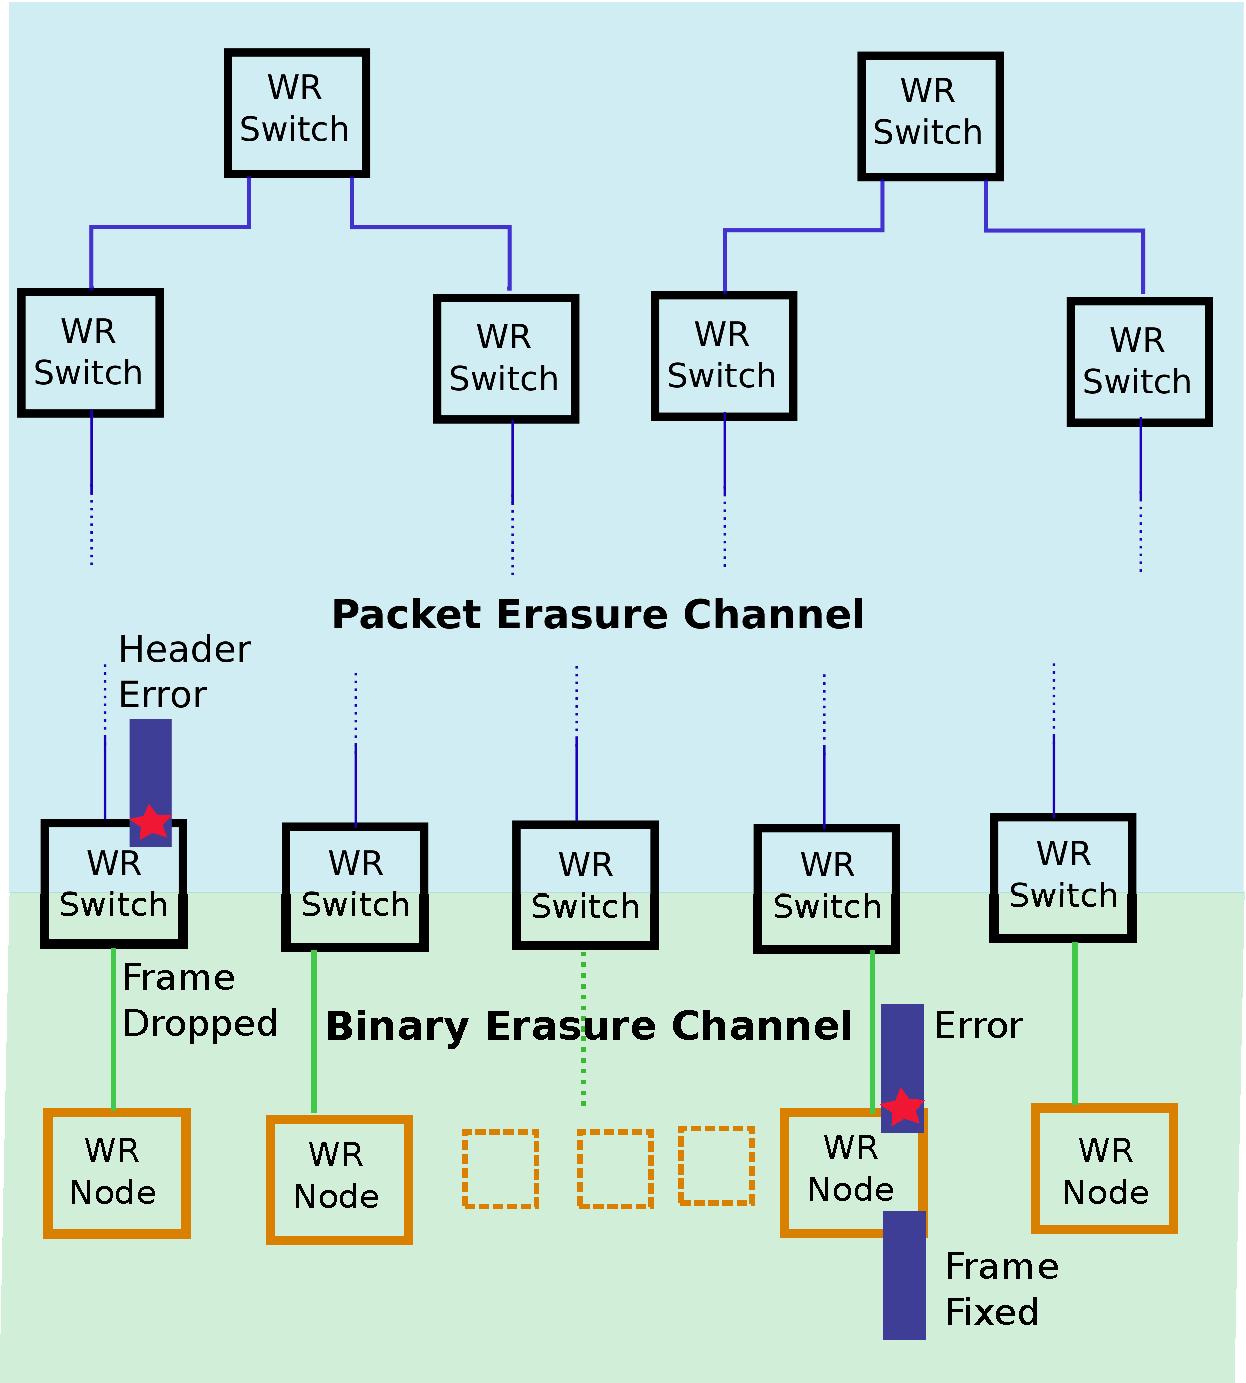
\includegraphics[scale=0.40]{../../../../figures/robustness/channels.ps}
	\captionof{figure}{PEC and BEC in a WR Network}
	\label{fig:wr_channels}
\end{center}

\subsection{Codes for Packet Erasure Channels}

Codes for PEC allows $k$ frames to be encoded into n encoded frames. The source
frames are encoded in such a way that the reception of any subset of $k$ encoded
frames at the receiver suffices to recover all the source frames. If more
than $n-k$ encoded frames are lost, recovery of all the source frames is not
possible.

\subsubsection{Reed Solomon}

Reed-Solomon codes can be used to perform a form of forward error correction FEC
in a switched networks. 
The encoding and decoding employs arithmetic in the $GF(2^m)$ domain. The
value m is the code word size of the encoding. 
The \ControlMessage\ is subdivided into code blocks of $m$ bits length and
check values must be computed for each code block. 
The frames transmitted consist of frames with \ControlMessage\ blocks and check
frames with redundant data used in reconstructing lost frames. 

The encoded frames of $n$ data and $k$ check frames where $n+k <= 2^m$. The
algorithm requires an encoding/decoding matrix of $n + k$ rows and $n$ columns.
The required matrix is derived from Vandermonde matrix which always generates
the first $k$ encoded frames to be identical to the $k$ blocks of source 
\ControlMessage. This simplifies the decoding of the encoded frames and the
recovery of the \ControlMessage.

We strongly encourage to follow the RFC 5510 \cite{reed_solomon} which
describes a Fully-Specific Forward Error Correction scheme for the Reed-Solomon
Error code over $GF(2^m)$, in case a compatible of FEC with other
systems is desired. Although for the time being, WR will not be compliant to
this RFC, such compliance is considered to make easier the interoperation of a
WR device with non-WR devices regarding FEC.

The Appendix~\ref{appFEC} presents the encoder/decoder algorithm. 

%\subsection{Codes for Binary Erasure Channel} 


\subsubsection{Single-Bit Correction Code, Hamming Code}

The aim of the Hamming code is to detect up to two simultaneous bit
errors, and correct single-bit error. In case of two or more errors the frame
will be drop by the WR Node. In a Hamming code, multiple parity-check bits are
included within the message. Any particular bit, whether part of the
message or just a parity bit, would have a unique combination of check-bits
associated with it. The information-bits and the check-bits are located at
particular locations in the frame. This pattern is followed in any Hamming code,
regardless how many check-bits are included. The other locations are used by
information bits. An encoded packet by a Hamming Code looks like:

\begin{equation}
	Frame =    p_1\;  p_2 \;  b_1 \;  p_3 \;  b_2 \;  b_3 \;  b_4 \;  p_1  \;  b_5 \; b_6  \; b_7 .... 
\end{equation}

with $p_i$ as a parity bit and $b_i$ as information bit. 


The number of parity bits (redundant information) for a given stream of bits is
shown in the Figure~\ref{fig:Hamming}.

For the shortest payload of an Ethernet frame, 46 bytes, the code will introduce
9 parity bits, and for the longest, 1500 bytes, 14 bits.

\begin{center}
        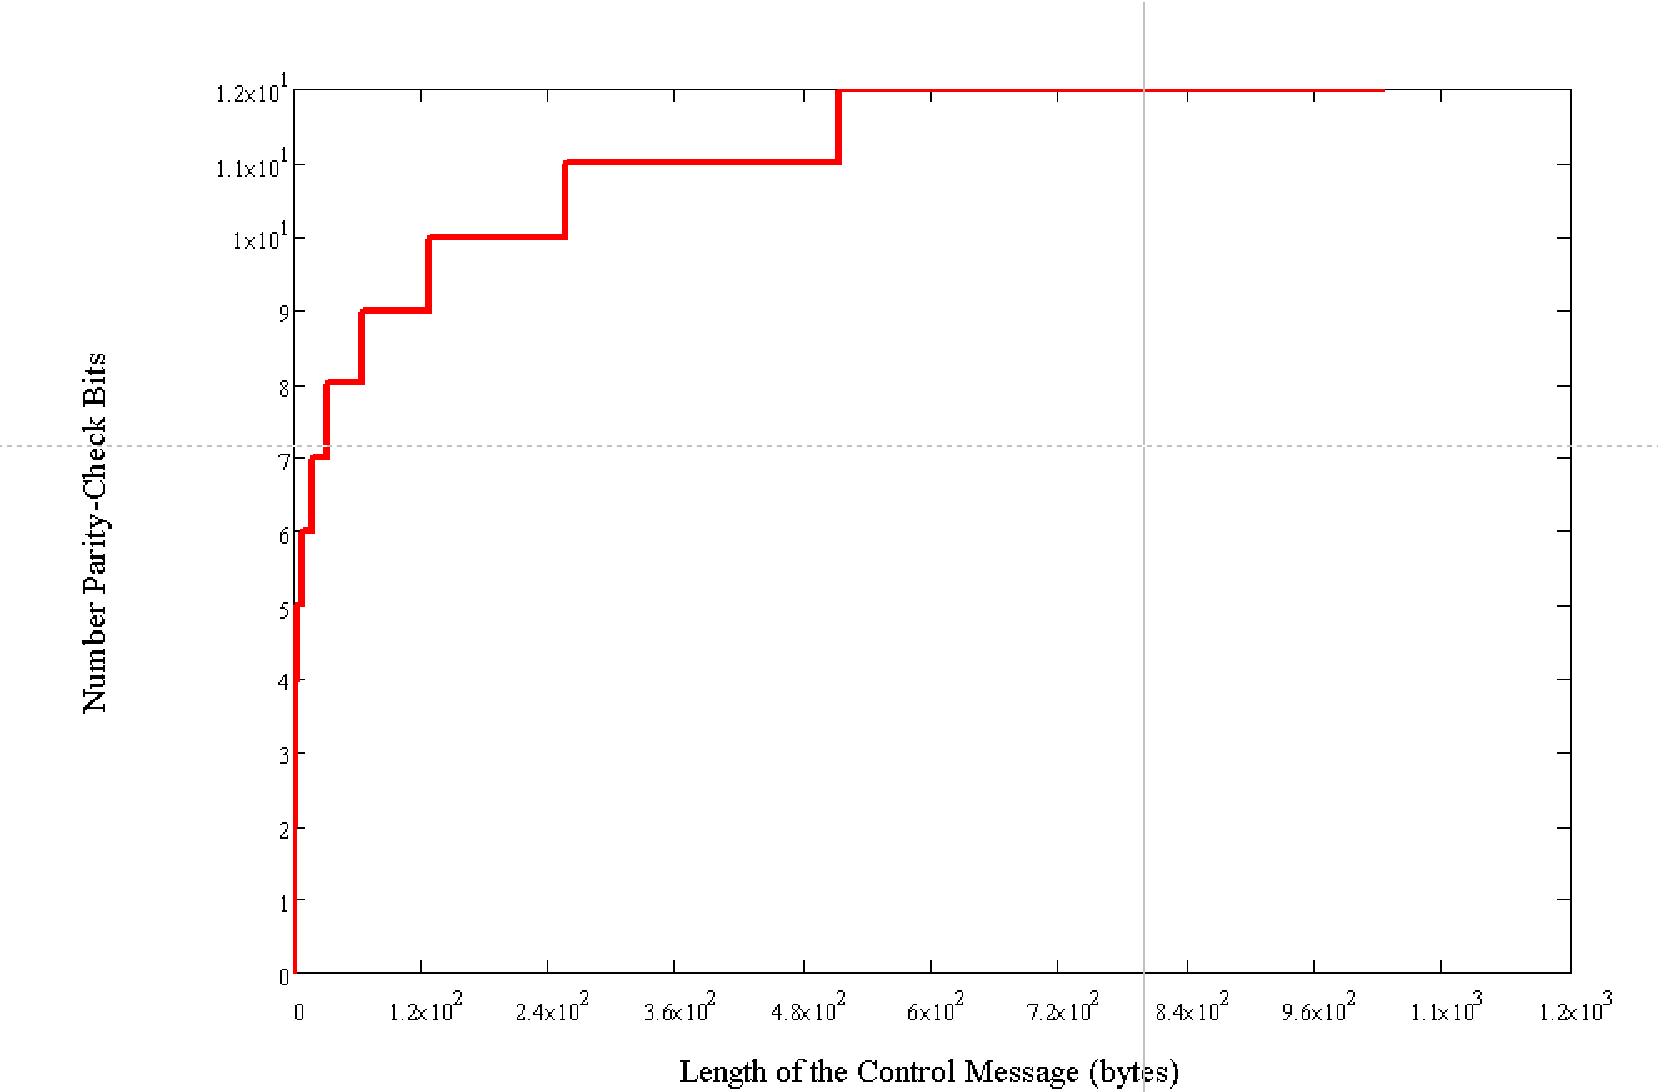
\includegraphics[scale=0.50]{../../../../figures/robustness/hamming.ps}
        \captionof{figure}{Number of Parity-Check bits for a given Control Message }
        \label{fig:Hamming}
\end{center}

In the Appendix~\ref{appFEC} we explain the general algorithm which generates a
single-error correcting code for any number of bits. 

\subsection{Multi-Bit Correction Code}

In the case that the global BER of the network is too high and one error
correction bit does not fulfil the requirements, there are other FEC that
could provide more corrections: LDPF, Reed Solomon, Raptor Code, Turbo
Code, etc.

\subsection{WR FEC Scheme}

So far we have presented two FEC mechanism to overcome the erasure and the loss of frames in the switches. Since both problems will occur in the WR network, the solution is to concatenate both FECs. The code for the BEC will add
redundant information to the \ControlMessage\ encoded into code blocks by the
PEC code. This will allow the Nodes to decode a frame if
it has single bit error. In the case that the node cannot decode the frame,
the frame is considered lost. However, the PEC decoder is able
to decode the \ControlMessage\ as long as it receivers N out M frames. Below we
present a systematic analysis of the scheme and we provide an analytical
expression to calculate the probability of loss of a \ControlMessage.


For a \ControlMessage\ $msg\_b$ we define the code block size $code\_block$

\begin{equation}
N_{code\_blocks} = ceil(\frac{msg\_b}{code\_block})
\end{equation}

in which, the PEC code will encode the information introducing an $overhead$
to the \ControlMessage\ with the aim of overcoming the loss of frames. Thus, the
\ControlMessage\ will be encode into blocks $N_{Code\_Blocks}$:

\begin{equation}
N_{e\_code\_blocks} = ceil(\frac{bits\_Control\_Message *overhead}{code\_block})
\end{equation}

wiht $N_{code\_blocks} \leq N_{e\_code\_blocks}$ and $ N_{e\_code\_blocks} =
N_{frames}$

\vspace{0.3 cm}

The BEC code will introduce redundant information, to the PEC-encoded code block
$rs\_cb\_b$ as depicted in Figure~\ref{fig:Hamming} $hamming_{rate}$.
This information that make up the payload of the Ethernet frame is:

\begin{equation}
bits\_payload = hamming_rate * length(code\_block)
\end{equation}

Thus, the probability of a packet dropped (in case of an error in the header of
the Ethernet frame) is:
\begin{equation}
P_{Error\_Header} = 1 - (1-BER)^{header\_bits}
\end{equation}

The probability of $n\_errors$ in the body, which can be repaired by the
BEC code, $max\_bits\_correctable$ is :

\begin{equation}
\footnotesize
P_{Error\_Payload} = 1 - \sum\limits_{n\_errors=0}^{max\_bits\_correctable}
\binom{bits\_payload} {n\_errors} BER^{n\_errors} \ (1-BER)^{bits\_payload -
n\_errors} BER^{n\_errors} \\
\end{equation}

then, the probability of a lost packet is:
\begin{equation}
P_{Frame\_Lost} = P_{Error\_Header} + P_{Error\_Payload} - (P_{Error\_Header} *
P_{Error\_Payload)}
\end{equation}

The probability that a control message cannot be decoded because of a lack of
sufficient encoded frames $N_{HP\_frames}$ or/and more errors than
$max\_bits\_correctable$ in the payload is: 

\begin{eqnarray}
P_{lost\_control\_message} & = & 1- \sum\limits_{n=0}^{N_{e\_code\_blocks}} - 
N_{code\_blocks} \dbinom{N_{e\_code\_blocks}}{n} \\ &&
*  (1 - P_{Packet\_Lost})^{N_{e\_code\_blocks}}\nonumber \\ && 
* P_{Packet\_Lost}^{n} \nonumber
\end{eqnarray}


$ Max\_Lost\_Control\_Message_{year} \leq  P_{lost\_control\_message} *
Control\_Message_{year} $

\vspace{0.3cm}

A WR network is made up of 2000 WR Receivers (Nodes). The connection among WR
Switches (16 ports) is established with fibre optic ($BER = 10^{-12}$),
and among the WR Switches and WR Nodes with UTP CAT-5 ($BER= 10^{-10}$). Hence,
the network will be interconnected using 2133 paths and a $BER_{broadcast} =
2.133 \ 10^{-9}$. We consider that one \ControlMessage\ will be sent per \GW. 

\begin{table}[!ht]
 	\begin{center}
\begin{tabular}{c|m{3cm}|m{3cm}|}
	\cline{2-3}
	&  \multicolumn{2}{|c|}{Use Case} \\ \cline{2-3}
	&  GSI & CERN \\ \hline
	\multicolumn{1}{|c|}{Control Message length} & $500$ & $1500$     \\ \hline
	\multicolumn{1}{|c|}{Control Message per year} & $3.145 10^{11} $ &$  3.145 10^{8} $ \\ \hline
	\multicolumn{1}{|c|}{Max Bit Correct.} & 1 & 1  \\ \hline
	\multicolumn{1}{|c|}{Parity-Check Bits} & 13    &  13   \\ \hline
	\multicolumn{1}{|c|}{PEC Code Overhead} & 3  & 2 \\ \hline
	\multicolumn{1}{|c|}{Payload Length} & 400 B  & 800b \\ \hline
	\multicolumn{1}{|c|}{Num Encoded Frames} & 4  & 4 \\ \hline
	\multicolumn{1}{|c|}{Needed Frames in Receiver} & 2 & 2 \\ \hline
	\multicolumn{1}{|c|}{Probability of Loosing a \ControlMessage} & $10^{-14}$ & $10^{-13}$\\ \hline
	\end{tabular}   
	\caption{GSI and CERN FEC characteristics}
	\label{tab:gsi_cern_fec}
	\end{center}
\end{table}

The values presented in the Table~\ref{tab:gsi_cern_fec} prove that the
concatenated FECs (BEC code and PEC code) guarantee that less than one
\ControlMessage per year will be lost. It's important to point out that only
single bit correction is sufficient to fulfill the requirement..
In the Appendix~\ref{app:wr_fec_graphs} the graphs for these two use
cases is presented.

\subsection{White Rabbit FEC Header}

All the frames encoded by the WR FEC scheme will contain in the very beginning
of the payload of the Ethernet frame a header with the following field:

\begin{itemize}
	\item Type of FEC scheme
	\item FEC frame ID, see Chapter~\ref{chap:CTRLdataMonitoring}
	\item Frame ID
\end{itemize}

\begin{center}
        
\includegraphics[scale=0.80]{../../../../figures/robustness/fec_header.ps}
        \captionof{figure}{WR FEC Header}
         \label{fig:fec_header}
\end{center}

Three bits in the header will indicate which kind of FEC is being used for the
frame.The FEC will create several Code Blocks from one \ControlMessage, those
will be enumerated for decoding process. Four bits are available for this
purpose. Also a unique FEC Frame ID will keep track of the encoded frames for
diagnostics.






